\documentclass[tikz,border=6pt]{standalone}
\usepackage[T1]{fontenc}
\usepackage[utf8]{inputenc}
\usepackage{pgfplots}
\usepgfplotslibrary{groupplots}
\usetikzlibrary{calc}
\pgfplotsset{compat=1.18}
\begin{document}
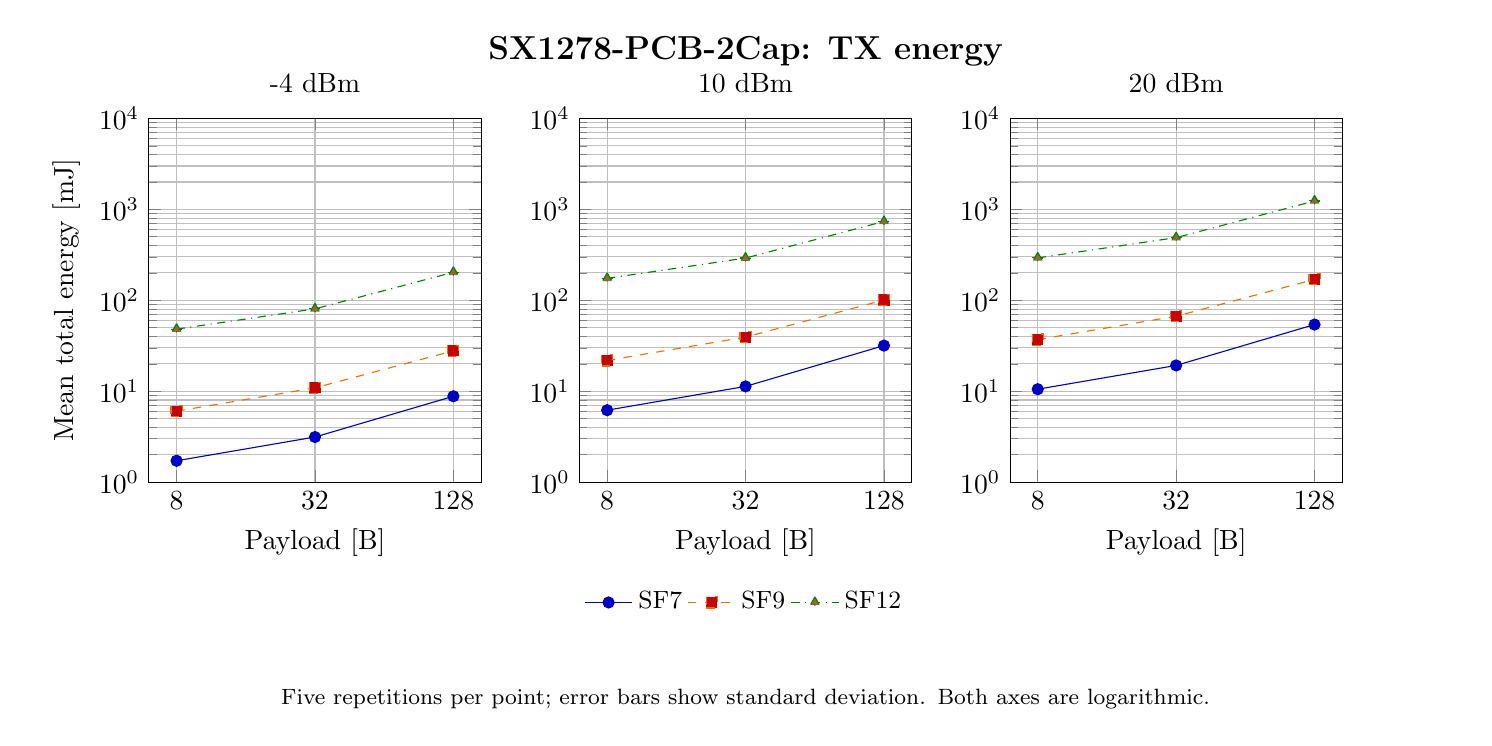
\begin{tikzpicture}
\begin{groupplot}[/pgf/number format/use comma, group style={group size=3 by 1, horizontal sep=1.25cm},
  width=5.8cm,height=6.2cm,xmode=log,log basis x=2,ymode=log,log basis y=10,ymin=1,ymax=10000,
  xtick={8,32,128},xticklabels={8,32,128},grid=both,xlabel={Payload [B]},
  legend style={draw=none,fill=none,font=\small,at={(0.5,-0.27)},anchor=north,legend columns=-1}]
% TX energy
\nextgroupplot[title={-4 dBm},ylabel={Mean total energy [mJ]}]
\addplot+[blue!75!black,solid,mark=*,error bars/.cd,y dir=both,y explicit] coordinates {(8,1.71615319) +- (0,0.00347312864) (32,3.13084623) +- (0,0.00911948384) (128,8.78737547) +- (0,0.00977237643)};
\addplot+[orange!90!black,dashed,mark=square*,error bars/.cd,y dir=both,y explicit] coordinates {(8,6.02751691) +- (0,0.0156011614) (32,10.8802158) +- (0,0.0164456904) (128,27.7962308) +- (0,0.0449625417)};
\addplot+[green!50!black,dashdotted,mark=triangle*,error bars/.cd,y dir=both,y explicit] coordinates {(8,48.1283972) +- (0,0.0416249322) (32,80.4039942) +- (0,0.034352442) (128,203.180825) +- (0,0.117724395)};
\nextgroupplot[title={10 dBm}]
\addplot+[blue!75!black,solid,mark=*,error bars/.cd,y dir=both,y explicit] coordinates {(8,6.17743141) +- (0,0.00452141343) (32,11.2868) +- (0,0.00954912678) (128,31.7385007) +- (0,0.00997065897)};
\addlegendentry{SF7}
\addplot+[orange!90!black,dashed,mark=square*,error bars/.cd,y dir=both,y explicit] coordinates {(8,21.7663612) +- (0,0.0125489421) (32,39.3066748) +- (0,0.0286183149) (128,100.623628) +- (0,0.0555729644)};
\addlegendentry{SF9}
\addplot+[green!50!black,dashdotted,mark=triangle*,error bars/.cd,y dir=both,y explicit] coordinates {(8,174.183139) +- (0,0.0160360288) (32,291.289852) +- (0,0.0860171793) (128,736.103968) +- (0,0.210911511)};
\addlegendentry{SF12}
\nextgroupplot[title={20 dBm}]
\addplot+[blue!75!black,solid,mark=*,error bars/.cd,y dir=both,y explicit] coordinates {(8,10.5149778) +- (0,0.0448558818) (32,19.1972084) +- (0,0.0789783074) (128,54.0580208) +- (0,0.245531543)};
\addplot+[orange!90!black,dashed,mark=square*,error bars/.cd,y dir=both,y explicit] coordinates {(8,37.0048645) +- (0,0.220095035) (32,66.7473383) +- (0,0.375907224) (128,169.713111) +- (0,0.688965257)};
\addplot+[green!50!black,dashdotted,mark=triangle*,error bars/.cd,y dir=both,y explicit] coordinates {(8,292.537555) +- (0,0.588519522) (32,488.72549) +- (0,0.595746087) (128,1237.13689) +- (0,2.3561846)};
\end{groupplot}
\node[font=\bfseries\large] at ($(group c2r1.north)+(0,0.85cm)$) {SX1278-PCB-2Cap: TX energy};
\node[font=\footnotesize,align=center,text width=18cm] at ($(group c2r1.south)+(0,-2.75cm)$) {Five repetitions per point; error bars show standard deviation. Both axes are logarithmic.};
\end{tikzpicture}
\end{document}
